% Created 2015-03-27 Fri 14:19
\documentclass[11pt]{article}
\usepackage[utf8]{inputenc}
\usepackage[T1]{fontenc}
\usepackage{fixltx2e}
\usepackage{graphicx}
\usepackage{longtable}
\usepackage{float}
\usepackage{wrapfig}
\usepackage{rotating}
\usepackage[normalem]{ulem}
\usepackage{amsmath}
\usepackage{textcomp}
\usepackage{marvosym}
\usepackage{wasysym}
\usepackage{amssymb}
\usepackage{hyperref}
\tolerance=1000
\usepackage[utf8]{inputenc}
\usepackage[usenames,dvipsnames]{color}
\usepackage[backend=bibtex, style=numeric]{biblatex}
\usepackage{commath}
\usepackage{tikz}
\usetikzlibrary{shapes,backgrounds}
\usepackage{marginnote}
\usepackage{listings}
\usepackage{color}
\usepackage{enumerate}
\hypersetup{urlcolor=blue}
\hypersetup{colorlinks,urlcolor=blue}
\addbibresource{bibliography.bib}
\setlength{\parskip}{16pt plus 2pt minus 2pt}
\definecolor{codebg}{rgb}{0.96,0.99,0.8}
\definecolor{codestr}{rgb}{0.46,0.09,0.2}
\author{Oleg Sivokon}
\date{\textit{<2015-03-27 Fri>}}
\title{Assignment 11, Introduction to Statistics}
\hypersetup{
  pdfkeywords={Discrete Mathematics, assignment, bar chart, histogram},
  pdfsubject={First asssignment in the course Introduction to Statistics},
  pdfcreator={Emacs 25.0.50.1 (Org mode 8.2.2)}}
\begin{document}

\maketitle
\tableofcontents


\lstset{ %
  backgroundcolor=\color{codebg},
  basicstyle=\ttfamily\scriptsize,
  breakatwhitespace=false,         % sets if automatic breaks should only happen at whitespace
  breaklines=false,
  captionpos=b,                    % sets the caption-position to bottom
  commentstyle=\color{mygreen},    % comment style
  framexleftmargin=10pt,
  xleftmargin=10pt,
  framerule=0pt,
  frame=tb,                        % adds a frame around the code
  keepspaces=true,                 % keeps spaces in text, useful for keeping indentation of code (possibly needs columns=flexible)
  keywordstyle=\color{blue},       % keyword style
  showspaces=false,                % show spaces everywhere adding particular underscores; it overrides 'showstringspaces'
  showstringspaces=false,          % underline spaces within strings only
  showtabs=false,                  % show tabs within strings adding particular underscores
  stringstyle=\color{codestr},     % string literal style
  tabsize=2,                       % sets default tabsize to 2 spaces
}

\clearpage

\section{Problems}
\label{sec-1}

\subsection{Problem 1}
\label{sec-1-1}
Given the grades in an engineering faculty were as follows:

\begin{center}
\begin{tabular}{rrr}
lower & higher & graded\\
\hline
30 & 60 & 15\\
60 & 75 & 45\\
75 & 85 & 45\\
85 & 100 & 15\\
\end{tabular}
\end{center}

\begin{enumerate}
\item Present the data using a histogram.
\item Calculate mode, median, algebraic average and variance.
\item Calculate the number of students who earned at least 82 points.
\item Given the following data for the preceding year for 80 students
where the average grade was 70 and variance was 200, find the
average and the variance for two years combined.
\end{enumerate}

\subsubsection{Answer 1}
\label{sec-1-1-1}

\lstset{language=R,label=students-histogram,numbers=none}
\begin{lstlisting}
library(ggplot2)
tbl$avg <- (tbl$lower + tbl$higher) / 2
ggplot(tbl) + 
    geom_histogram(
        aes(x = avg, weight = graded, fill = ..count..), 
        breaks = unique(append(tbl$lower, tbl$higher)),
        position = "identity", colour = "black") +
            xlab("grades")
\end{lstlisting}

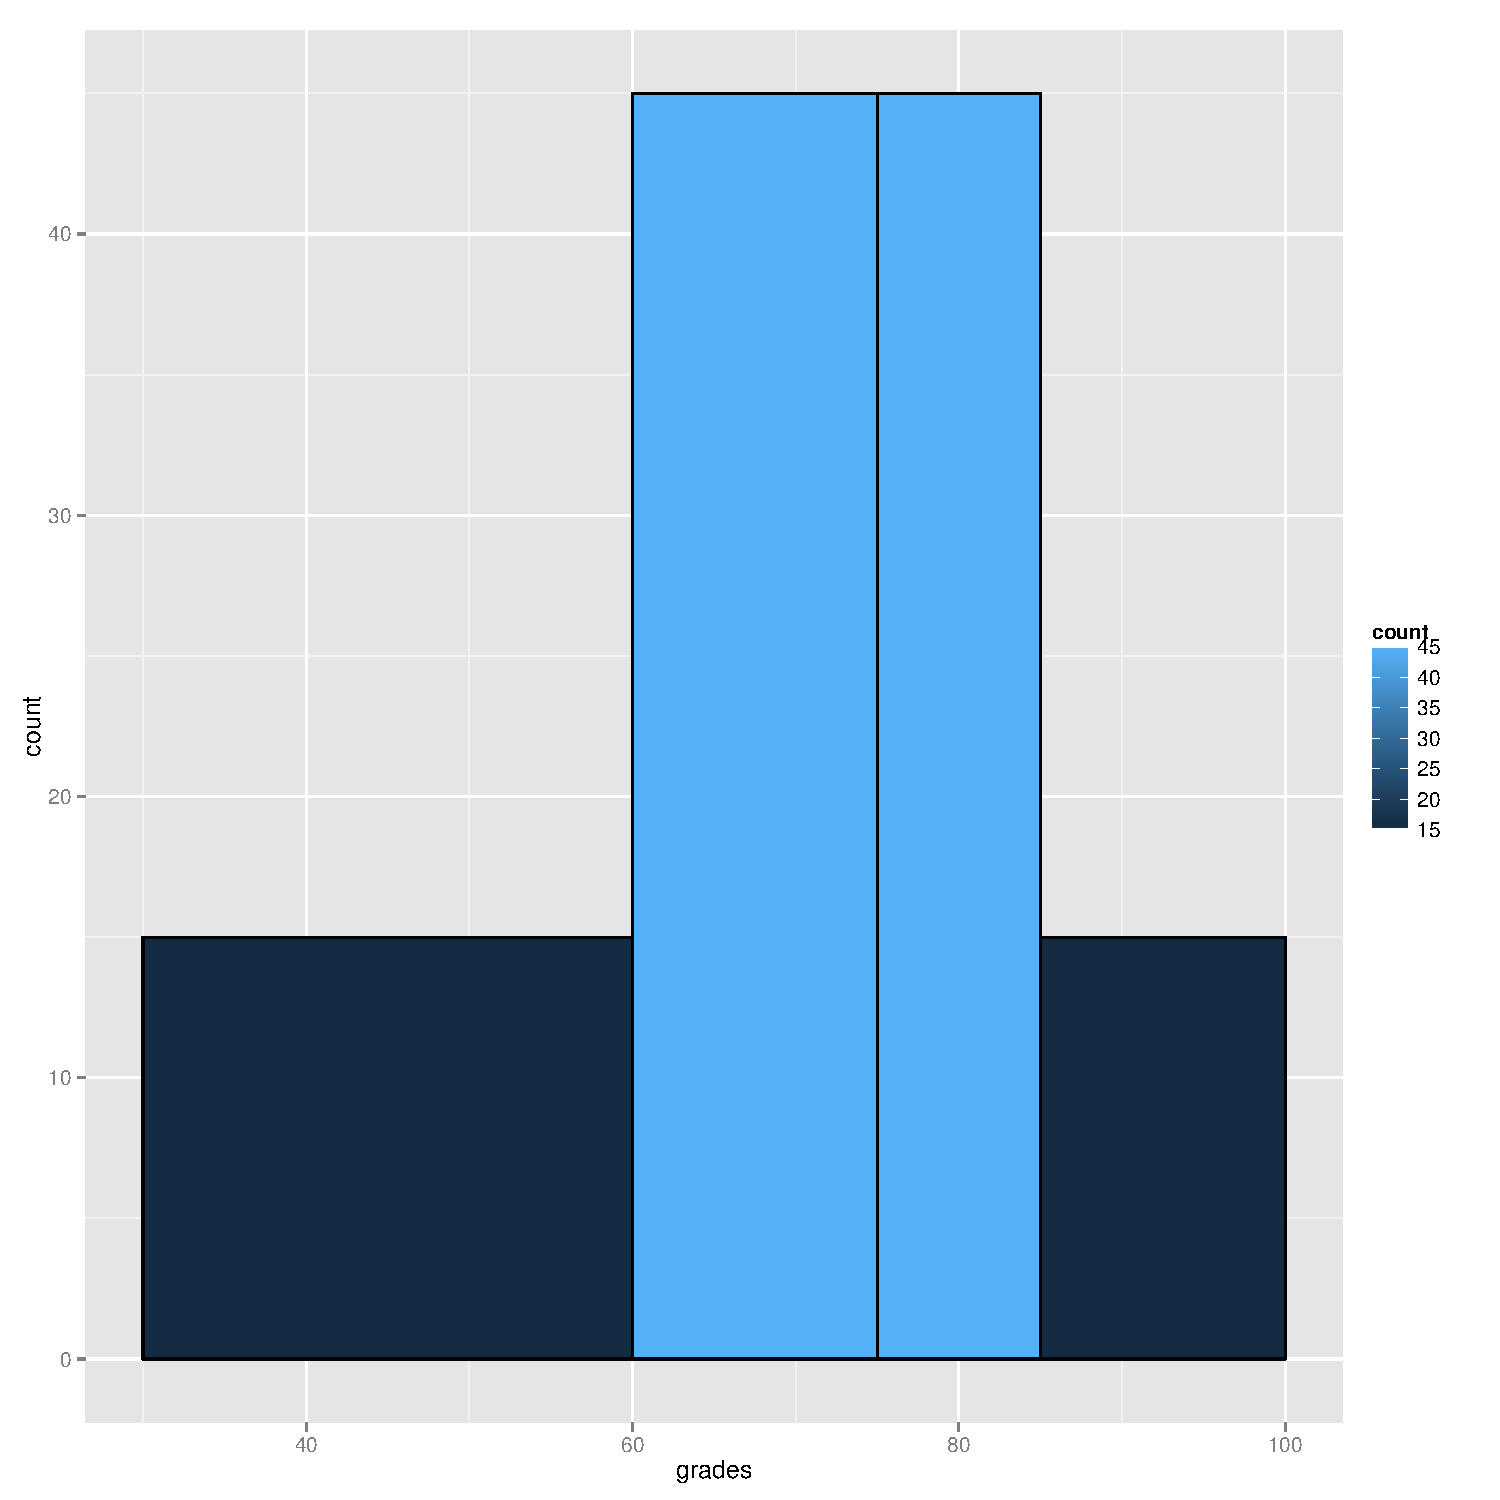
\includegraphics[width=.9\linewidth]{images/students.pdf}
\subsubsection{Answer 2}
\label{sec-1-1-2}
As easy to see from the diagram, there are two \textbf{modes}: one is in the
(60, 75] range, an another is in the (75, 85] range.

The \textbf{median} is the value at the 60'th studen, which is easy to see
from the table as being the 75 points.
\begin{equation*}
  \begin{aligned}
    Md &= \frac{\frac{n}{2} - F(x_{m-1})}{f(x_m)} * (L_1-L_0)+L_0 \\
    Md &= \frac{\frac{120}{2} - 60}{45} * (85 - 75) + 75 \\
    Md &= \frac{60 - 60}{45} * (85 - 75) + 75 \\
    Md &= 75
  \end{aligned}
\end{equation*}

The \textbf{average} is given by the formula:
\begin{equation*}
  \begin{aligned}
    \frac{15 * \frac{30 + 60}{2} + 45 * \frac{60 + 75}{2} +
      45 * \frac{75 + 85}{2} + 15 * \frac{85 + 100}{2}}{15 + 45 + 45 + 15} = \\
    \frac{15 * 90 + 45 * 135 + 45 * 160 + 15 * 185}{2 * 120} = \\
    \frac{17400}{240} = \\72.5
  \end{aligned}
\end{equation*}

And the \textbf{variance}:
\begin{equation*}
  \begin{aligned}
    S^2 &= \frac{\sum_1^n (x - \overline{x})^2 * f(x)}{n} \\
    S^2 &= \frac{(45 - 72.5)^2 * 15 + (67.5 - 72.5)^2 * 45 +
      (80 - 72.5)^2 * 45 + (92.5 - 72.5)^2 * 15}{120} \\
    S^2 &= \frac{756.25 * 15 + 25 * 45 + 56.25 * 45 + 400 * 15}{120} \\
    S^2 &= \frac{21000}{120} \\
    S^2 &= 175
  \end{aligned}
\end{equation*}
% Emacs 25.0.50.1 (Org mode 8.2.2)
\end{document}